\documentclass[border=5pt]{standalone}
\usepackage{tikz}
\usepackage{amsmath}
\begin{document}
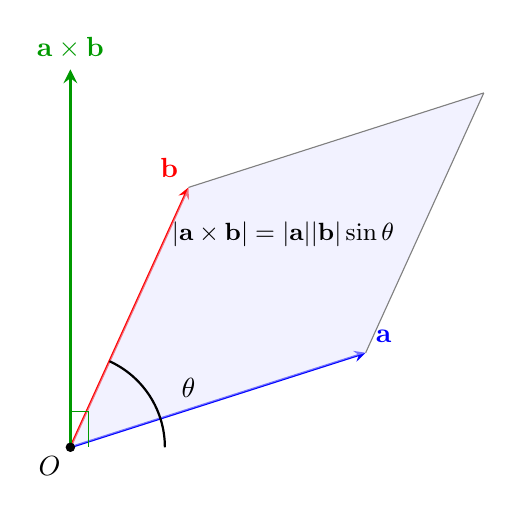
\begin{tikzpicture}[scale=1.5, >=stealth]
  % 3D coordinate system (isometric projection)
  \pgfmathsetmacro{\ang}{25}  % angle for 3D effect

  % Vectors a and b
  \draw[->, thick, blue] (0,0) -- (2.5, 0.8) node[above right] {$\mathbf{a}$};
  \draw[->, thick, red] (0,0) -- (1.0, 2.2) node[above left] {$\mathbf{b}$};

  % Cross product a × b (perpendicular to both, coming "out" of plane)
  \draw[->, very thick, green!60!black] (0,0) -- (0, 3.2) node[above] {$\mathbf{a} \times \mathbf{b}$};

  % Parallelogram formed by a and b
  \fill[blue!10, opacity=0.5] (0,0) -- (2.5,0.8) -- (3.5,3.0) -- (1.0,2.2) -- cycle;
  \draw[gray, thin] (2.5,0.8) -- (3.5,3.0);
  \draw[gray, thin] (1.0,2.2) -- (3.5,3.0);

  % Angle between a and b
  \draw[thick] (0.8,0) arc (0:{atan2(2.2,1.0)}:0.8);
  \node at (1.0, 0.5) {$\theta$};

  % Right angle symbol at origin for a×b vs a
  \draw[green!60!black, thin] (0, 0.3) -- (0.15, 0.3) -- (0.15, 0);

  % Labels
  \node[font=\small] at (1.8, 1.8) {$|\mathbf{a} \times \mathbf{b}| = |\mathbf{a}||\mathbf{b}|\sin\theta$};

  % Origin
  \filldraw[black] (0,0) circle (1pt) node[below left] {$O$};
\end{tikzpicture}
\end{document}
